% Messwerte: Alle gemessenen Größen tabellarisch darstellen
% Auswertung: Berechnung geforderter Ergebnisse mit Schritten/Fehlerformeln/Erläuterung/Grafik (Programme)
\section{Auswertung}
\label{sec:auswertung}

\subsection{Fehlerrechnung}
\label{sec:Fehlerrechnung}

%\subsection{Formeln für den Mittelwert, den Gauß-Fehler und die Standardabweichung }
%\label{sec:Formeln fuer den Mittelwert, den Gauss-Fehler und die Standardabweichung}
    Für den Mittelwert gilt
    \begin{equation}
    \bar{x} = \frac{1}{N}\sum\limits_{i = 1}^N x_i .
    \end{equation}

    Für den Fehler des Mittelwertes gilt
    \begin{equation}
        \Delta \bar{x}=\frac{1}{\sqrt{N}} \sqrt{\frac{1}{N-1} \sum_{i=1}^N\left(x_i-\bar{x}\right)^2}.
        \label{eqn:mittelwert}
        \end{equation}

    Für die Gaußsche Fehlerfortpflanzung gilt

    \begin{equation}
        \Delta f=\sqrt{\sum_{i=1}^N\left(\frac{\partial f}{\partial x_i}\right)^2 \cdot\left(\Delta x_i\right)^2}.
    \end{equation}

    Diese Formeln werden für sämtliche Fehlerrechnungen in diesem Versuch verwendet, ohne sie für die 
    jeweiligen Rechnungen explizit anzugeben. Die Rechnungen selbst werden dabei mithilfe von
    Uncertainties durchgeführt.

\subsection{Durchlasskurve}
\label{sec:Durchlasskurve}

Zunächst wird die Filterkurve eines Selektivverstärkers untersucht, wobei eine effektive Spannung $U_E$ in Höhe von $ \SI{1}{\volt}$ 
verwendet. Aufgenommen wird dabei die Ausgangspannung $U_A$ in Anhängigkeit von der Frequenz $v$. Die Frequenz wurde von $\SI{2}{\kHz}$ auf 
$\SI{31}{\kHz}$ hochgedreht. In der \eqref{tab:filterkurve} sind die aufgenommen Messwerte aufgetragen.

\begin{table}[H]
    \centering
    \caption{Die Messwerte für Filterkurve}
    \label{tab:filterkurve}
\begin{tabular}{c c}
    \toprule
          $v \, /\,\si{kHz}$ & $U \,/\,\si{v}$ \\
    \midrule
           2 &    0.01 \\
           4 &    0.02 \\
           6 &   0.025 \\
           8 &    0.03 \\
          10 &    0.04 \\
          11 &    0.05 \\
          12 &    0.06 \\
          13 &    0.07 \\
          14 &    0.08 \\
          15 &   0.095 \\
          16 &   0.115 \\
          17 &   0.145 \\
          18 &    0.19 \\
          19 &    0.26 \\
          20 &    0.42 \\
        20.5 &     0.6 \\
          21 &    0.98 \\
        21.1 &     1.2 \\
        21.2 &     1.3 \\
        21.3 &     1.5 \\
        21.4 &    1.85 \\
        21.5 &    2.35 \\
        21.6 &     3.1 \\
        21.7 &       4 \\
        21.8 &     4.4 \\
        21.9 &     3.8 \\
          22 &    2.95 \\
        22.1 &    2.45 \\
        22.2 &    1.85 \\
        22.3 &    1.55 \\
        22.4 &     1.3 \\
        22.5 &    1.15 \\
          23 &    0.68 \\
          25 &   0.265 \\
          27 &    0.17 \\
          29 &   0.125 \\
          31 &    0.1 \\
    \bottomrule
    \end{tabular}
\end{table}

In der \eqref{fig:plot} wird die Durchlasskurve der aufgenommenen Messwerte abgebildet.
Dabei ist der Quotient $\frac{U_A}{U_E}$ gegen die Frequenz $v$ aufgetragen. Anhand des Graphens lässt sich ablesen, dass das 
Maximum bei $\SI{21.8}{kHz}$ liegt mit einer Spannung von $\SI{4.4}{\volt}$. Dieses Maximum ist dann die Durchlassfrequenz.

\begin{figure}[H]
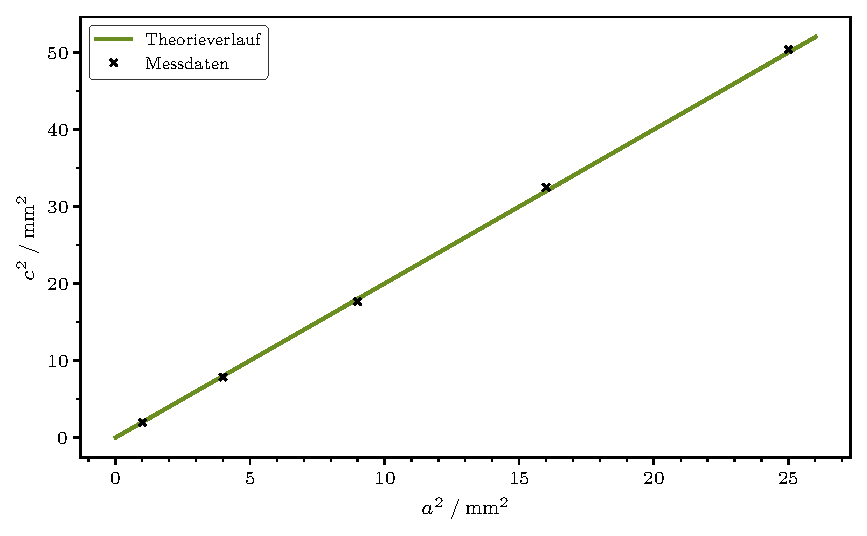
\includegraphics{build/plot.pdf}
	\caption{Filterkurve des Selektivverstärkers mit einer Güte $Q = 20$ und die Ausgleichskurve in Form einer Gaußverteilung .}
	\label{fig:plot}
\end{figure}

\subsection{Effektiver Querschnitt}
\label{sec:Effektiver Querschnitt}

Der effektive Querschnitt wird im Folgenden von vier unterschiedlioche Stoffe bestimmt.
Für die Berechnung des realen Querschnitts gilt 
\begin{equation}
  Q_{real}=\frac{m}{l \cdot \rho_w}.
\end{equation}

In der \eqref{tab:quer}stehen die gemessenen Werte für die Stoffe ,sowie die brechneten effektiven Querschnitte.

\begin{table}
  \centering
  \caption{Maße der Stoffe und der daraus berechnete effektive Querschnitt}
  \label{tab:quer}
\begin{tabular}{c c c c c}
  \toprule
  Stoff &  $m / \si{g}$ &  $l / \si{cm}$ &  $\rho / \si{g} \cdot \si{cm}^3$ & $Q / \si{cm}^2$ \\
  \midrule
  $Dy_2O_3$ & 14,38 &  16,3 &           7,80 & 0,113104 \\
  $Gd_2O_3$ & 14,08 &  17,3 &           7,40 & 0,109983 \\
  $Nd_2O_3$ & 18,48 &  14,5 &           7,24 & 0,176034 \\
  \bottomrule
  \end{tabular}
\end{table}


\subsection{Suszeptibilität}
Im Folgenden wird die Suszeptibilität $\chi$ unterschiedlicher Stoffe untersucht.

In der Tabelle \eqref{tab:dy} sind die Messwerte der Probe $Dy_2O_3$ angegeben. Es sind die 
Werte ohne die Probe für die Spannung und den Widerstand angebenen und für den Fall, dass die Probe
verwendet wurde. Daraus wurde die Differenz des Widerstände $\Delta R\mathbin{/}\si{\ohm}$ berechnet.

\begin{table}
  \centering
  \caption{Messwerte der Probe $Dy_2O_3$ sowie die Differenz $\Delta R$.}
  \label{tab:dy}
\begin{tabular}{c c | c c | c}
  \hline
  \multicolumn{2}{c}{ohne Probe} & \multicolumn{3}{c}{mit Probe} \\
  \hline
  $U\mathbin{/} \si{\mV}$ & $R_{3/4}\mathbin{/} \si{\ohm}$ & $U\mathbin{/} \si{\mV}$ & $R_{3/4}\mathbin{/} \si{\ohm}$ & $\Delta R\mathbin{/}\si{\ohm}$ \\
  \hline
  15.5  & 2.62 & 15    & 3.265 & 0.645\\
  16  & 2.565 & 15.5   & 3.245 & 0.68\\
  16.5 & 2.445 & 15   & 3.245 & 0.8\\
  16  & 2.525 & 14.3   & 3.245 & 0.72\\
  \bottomrule
  \end{tabular}
\end{table}

Aus den brechneten Werten der Differenz wird anschließend der Mittelwert \eqref{eqn:mittelwert} bestimmt
\begin{equation*}
  \bar{\Delta R} \approx 0.711 \si{\ohm}.
\end{equation*}
Ebenfalls wird der Mittelwert für den abgleich Widerstand $R_{3/4}$ ohne Probe gebildet
\begin{equation}
  \bar{R_{3/4}} \approx 2.539.
\end{equation}

Die Tabelle \eqref{tab:gd} beinhaltet die Messwerte für den Stoff $Gd_2O_3$. Die Werte für die Spannung und die Widerstände
vor dem Einführen und nach dem Einführen sind angegeben. Daraus wurde dann die Differenz der Widerstände brechnet. 
\begin{table}
  \centering
  \caption{Messwerte der Probe $Gd_2O_3$ sowie die Differenz $\Delta R$.}
  \label{tab:gd}
\begin{tabular}{c c | c c | c}
  \hline
  \multicolumn{2}{c}{ohne Probe} & \multicolumn{3}{c}{mit Probe} \\
  \hline
  $U\mathbin{/} \si{\mV}$ & $R_{3/4}\mathbin{/} \si{\ohm}$ & $U\mathbin{/} \si{\mV}$ & $R_{3/4}\mathbin{/} \si{\ohm}$ & $\Delta R\mathbin{/}\si{\ohm}$ \\
  \hline
  15.4 & 2.45 & 15.4  & 1.765 & 0.685\\
  16  & 2.48 & 15  & 1.73 & 0.75\\
  16 & 2.525& 15.4  & 1.775 & 0.75\\
  \bottomrule
  \end{tabular}
\end{table}

Für den Mittelwert der Widerstandsdifferenzen für den Stoff $Gd_2O_3$ ergibt sich
\begin{equation*}
  \bar{\Delta R} \approx 0.728 \si{\ohm}.
\end{equation*}
Ebenfalls wird der Mittelwert für den abgleich Widerstand $R_{3/4}$ ohne Probe gebildet
\begin{equation}
  \bar{R_{3/4}} \approx 2.485\si{\ohm}.
\end{equation}

Für den dritten Stoff wurde die gleiche Messung durchgeführt. Die Ergebnisse werden in \eqref{tab:nd}
abgebildet. Die Differenz wurde ebenfalls berechnet und in der Tabelle \eqref{tab:nd} abgebildet.
\begin{table}
  \centering
  \caption{Messwerte der Probe $Nd_2O_3$ sowie die Differenz $\Delta R$.}
  \label{tab:nd}
\begin{tabular}{c c | c c | c}
  \hline
  \multicolumn{2}{c}{ohne Probe} & \multicolumn{3}{c}{mit Probe} \\
  \hline
  $U\mathbin{/} \si{\mV}$ & $R_{3/4}\mathbin{/} \si{\ohm}$ & $U\mathbin{/} \si{\mV}$ & $R_{3/4}\mathbin{/} \si{\ohm}$ & $\Delta R\mathbin{/}\si{\ohm}$ \\
  \hline
  15.5 & 2.495 & 16.5  & 2.365 & 0.13\\
  17  & 2.535 & 16.5  & 2.265 & 0.27\\
  16 & 2.47& 16 & 2.30 & 0.17\\
  \bottomrule
  \end{tabular}
\end{table}

Für den Mittelwert der Widerstandsdifferenzen für den Stoff $Nd_2O_3$ ergibt sich
\begin{equation*}
  \bar{\Delta R} \approx 0.19 \si{\ohm}.
\end{equation*}
Ebenfalls wird der Mittelwert für den abgleich Widerstand $R_{3/4}$ ohne Probe gebildet
\begin{equation}
  \bar{R_{3/4}} \approx 2.5\si{\ohm}.
\end{equation}

Mit Hilfe der Formel %\eqref{eqn:}
lässt sich für die einzelnen Stoffe der experimentelle Wert der Suszeptibilität bestimmen.
Die berechneten Werte der einzelen Stoffe stehen in der Tabelle \eqref{tab:sus}.
\begin{table}
  \centering
  \caption{Die experimentell bestimmten Suszeptibilitäten}
  \label{tab:sus}
\begin{tabular}{c|c}
  \toprule
  Stoff & $\Chi$ \\
  \midrule
  $Dy_2O_3$ & 4.288\\
  $Gd_2O_3$ & 4.613\\
  $Nd_2O_3$ & 0.748\\
  \bottomrule
 \end{tabular}
\end{table}
